% !TeX root = proyecto.tex
% !TeX program = pdflatex
\documentclass[11pt,letterpaper]{article}

\usepackage[utf8]{inputenc}
\usepackage[T1]{fontenc}
\usepackage[spanish,es-nodecimaldot]{babel}
\usepackage{lmodern}
\usepackage[margin=2.3cm]{geometry}
\usepackage{amsmath}
\usepackage{amssymb}
\usepackage{booktabs}
\usepackage{array}
\usepackage{tabularx}
\usepackage{graphicx}
\usepackage{float}
\usepackage{enumitem}
\usepackage{microtype}
\usepackage{setspace}
\usepackage{titlesec}

\addto\captionsspanish{\renewcommand{\tablename}{Tabla}}

\setstretch{1.08}
\setlength{\parindent}{0pt}
\setlength{\parskip}{0.45em}
\setlist[itemize]{leftmargin=1.4em,itemsep=0.2em,topsep=0.2em}
\setlist[enumerate]{leftmargin=1.6em,itemsep=0.25em,topsep=0.2em}
\titleformat{\section}{\large\bfseries}{\thesection.}{0.5em}{}
\titleformat{\subsection}{\normalsize\bfseries}{\thesubsection.}{0.5em}{}
\titlespacing*{\section}{0pt}{1.2em}{0.35em}
\titlespacing*{\subsection}{0pt}{0.9em}{0.25em}

\newcommand{\far}{\mathrm{FAR}}
\newcommand{\frr}{\mathrm{FRR}}
\newcommand{\auc}{\mathrm{AUC}}
\graphicspath{{figuras/}}

\begin{document}

\begin{titlepage}
  \thispagestyle{empty}
  \centering
  {\large\bfseries MAESTRÍA EN INTELIGENCIA ARTIFICIAL\par}
  \vspace{0.35cm}
  {\large MATEMÁTICAS Y PROGRAMACIÓN PARA IA\par}
  \vspace{1.8cm}
  \rule{\textwidth}{1.1pt}\par
  \vspace{0.8cm}
  {\LARGE\bfseries
    Detección temprana de suplantación durante una sesión activa mediante dinámica de mouse\par
  }
  \vspace{0.55cm}
  {\large
    Estudio de caso con autenticación continua y detección de anomalías\par
  }
  \vspace{0.8cm}
  \rule{\textwidth}{1.1pt}\par
  \vfill
\end{titlepage}
\pagenumbering{arabic}

\begin{abstract}
Los controles de acceso tradicionales verifican credenciales en un instante, pero no garantizan que la persona
que continúa operando una sesión sea quien se autenticó. Este trabajo estudia la dinámica de mouse como una
biometría conductual para detectar cambios de operador mientras la sesión permanece activa. La propuesta se
fundamenta en tres ideas: el movimiento voluntario presenta regularidades cinemáticas, cada persona conserva a la
vez variación motora natural y la interacción con el mouse permite construir perfiles no intrusivos. Se realiza un
estudio de caso con \texttt{user12} del conjunto Balabit. Un \emph{Isolation Forest} se ajusta solo con ventanas
legítimas; el umbral se fija con validación legítima y la prueba usa los primeros 25, 50, 75, 100, 125 o 150 eventos
de cada sesión. El mejor compromiso se observó con 100 eventos, con $\auc=0.692$, $\far=69.4\%$ y
$\frr=3.6\%$. Ningún tamaño satisfizo simultáneamente el criterio previo de $\auc\geq0.80$,
$\far\leq10\%$, $\frr\leq10\%$ y cobertura total. Por tanto, el experimento identifica señales útiles,
especialmente relacionadas con la aceleración, pero no valida todavía un autenticador operativo.
\end{abstract}

\textbf{Palabras clave:} autenticación continua, biometría conductual, dinámica de mouse, detección de anomalías,
suplantación de identidad.

\section{Introducción y contexto}

La autenticación mediante contraseña, código de un solo uso o biometría física suele concentrarse en el ingreso al
sistema. Una credencial correcta demuestra que alguien superó ese control, pero no que el mismo operador permanezca
frente al equipo durante toda la sesión. Una cuenta puede quedar abierta, ser cedida o pasar a manos de otra persona
después del acceso. También puede ser controlada por un programa o por un agente de inteligencia artificial capaz de
interactuar con la interfaz. El problema de este trabajo no es volver a comprobar una credencial, sino buscar evidencia
temprana de que cambió la forma de operar.

Este objetivo es distinto del de un CAPTCHA. Un CAPTCHA plantea un reto puntual para estimar si quien responde parece
ser humano. La autenticación continua, en cambio, compara una secuencia de comportamiento con el perfil previamente
registrado de una persona concreta. La dinámica de mouse puede, por ello, señalar tanto a otro ser humano como a un
sistema automatizado cuando su patrón se aparta del perfil legítimo. Sin embargo, una anomalía no identifica su
causa:
no demuestra por sí sola que exista mala intención ni permite afirmar que el operador sea una IA. En una aplicación
real, la alarma debería activar una verificación adicional y no una acusación automática.

\subsection{Base científica del comportamiento motor}

Cuando una persona mueve el mouse, el computador solo guarda una secuencia de datos: en qué momento ocurrió cada
evento, dónde estaba el puntero y si hubo un clic. Sin embargo, detrás de esos datos existe una acción humana. La
persona mira la pantalla, decide hacia dónde ir y coordina la mano y el brazo para llegar al objetivo. En ese
proceso toma muchas decisiones pequeñas: iniciar rápido o despacio, seguir una línea recta o una curva,
corregir la dirección, hacer una pausa y presionar el botón. Esas decisiones no se repiten de manera idéntica,
pero tampoco son totalmente
aleatorias.

Una comparación sencilla es la escritura a mano. Dos firmas de la misma persona nunca son exactamente iguales,
aunque suelen compartir rasgos de velocidad, tamaño, inclinación y presión. Con el mouse ocurre algo parecido. El
proyecto no busca una trayectoria idéntica que funcione como contraseña. Busca tendencias que aparecen muchas veces
y que, juntas,
pueden describir la forma habitual de interactuar de un usuario.

La cinemática es la parte de la física que describe cómo cambia un movimiento con el tiempo. No intenta explicar qué
músculo produjo el movimiento ni qué fuerza se aplicó, sino lo que puede observarse en el recorrido. En el caso del
mouse, la posición indica dónde está el puntero mediante las coordenadas $(x,y)$ y la trayectoria reúne todas esas
posiciones para mostrar el camino completo. Ese camino puede ser recto, curvo o incluir pequeñas correcciones cuando
la persona se desvía y vuelve a apuntar hacia su objetivo.

La velocidad indica cuánta distancia recorre el puntero durante un intervalo de tiempo. Si una persona mueve el mouse
una distancia grande en poco tiempo, la velocidad es alta; si recorre poca distancia en el mismo tiempo, la velocidad
es baja. La aceleración indica cómo cambia esa velocidad. Aparece cuando el usuario comienza a moverse, gana rapidez,
reduce la marcha o se detiene antes de llegar a un botón. También se observa cuánto gira el recorrido entre un tramo
y el siguiente. Las pausas, los clics y estos cambios de dirección ayudan a describir el ritmo con el que la persona
observa la pantalla, decide y actúa.

Flash y Hogan \cite{flash1985} estudiaron movimientos del brazo entre dos puntos y observaron que una persona no suele
mover la mano a velocidad constante. Normalmente comienza despacio, acelera, alcanza una velocidad máxima y vuelve a
reducirla al acercarse al destino. Cuando la velocidad se representa a lo largo del tiempo, el resultado suele parecer
una campana. También observaron que la mano tiende a reducir la velocidad en las partes más curvas del recorrido.

Para explicar ese comportamiento propusieron el modelo de mínimo \emph{jerk}\footnote{El \emph{jerk} es la rapidez
con la que cambia la aceleración; un valor alto indica un cambio brusco y uno bajo, un movimiento más suave.}. La idea
del modelo es que muchos movimientos voluntarios pueden aproximarse como una búsqueda de suavidad. Esto ayuda a
entender por qué la forma del camino, la velocidad y la aceleración no son números arbitrarios: reflejan cómo se
organiza el movimiento.

El estudio de Flash y Hogan no demostró que cada persona tenga una firma de mouse única. Además, sus experimentos
analizaron movimientos del brazo en condiciones controladas, no sesiones de computadora. El proyecto se basa en
principios de este tipo para elegir variables con significado físico, como la media y la variación de la aceleración.
Estas medidas se relacionan con la suavidad del movimiento, aunque no corresponden al cálculo directo del
\emph{jerk}.

Dhawale, Smith y Ölveczky \cite{dhawale2017} explican que ninguna persona repite un movimiento de forma idéntica. Una
parte de la variación proviene de pequeños cambios inevitables en el sistema nervioso y en los músculos. Otra parte
puede aparecer porque la persona aprende, se adapta o prueba una forma diferente de alcanzar el mismo objetivo. En el
uso de una computadora también pueden influir la tarea, la fatiga, el estado de ánimo, la superficie, la sensibilidad
del mouse o el dispositivo utilizado.

Las diferencias que aparecen entre movimientos de una misma persona reciben el nombre de variación intrausuario. Las
diferencias entre personas se conocen como variación interusuario. La autenticación solo puede funcionar bien cuando
las diferencias entre el propietario y los impostores son mayores que los cambios normales del propio usuario. Si el
modelo espera que el propietario se mueva siempre de la misma manera, generará alarmas cada vez que este cambie de
ritmo. Por eso el perfil debe representar varios comportamientos legítimos y no una única trayectoria ideal.

\newpage
La relación entre estas ideas y la seguridad informática aparece en el estudio de Antal y Egyed-Zsigmond
\cite{antal2019}. Los autores estudiaron la dinámica de mouse con el mismo conjunto Balabit utilizado en este
proyecto. Los datos se recogieron durante el uso general de una computadora y no mediante una sola tarea de
laboratorio. El movimiento se dividió en acciones, como mover, apuntar y hacer clic, o arrastrar un objeto. Después se
calcularon medidas de tiempo, distancia, velocidad, aceleración, dirección y suavidad.

Su resultado principal para este trabajo es que una sola acción contiene poca evidencia. En la parte más difícil de
su evaluación, el AUC pasó de aproximadamente 0.79 con una acción a 0.90 al combinar 20 acciones. Al utilizar
sesiones completas alcanzaron un AUC de 0.92. También observaron que varias medidas de aceleración y suavidad
aportaban más
información que algunas medidas simples de velocidad. Esto respalda la idea de acumular interacción antes de decidir.

Una acción del estudio de Antal y Egyed-Zsigmond reúne varios registros consecutivos; no equivale a un evento o fila
individual del conjunto de datos utilizado en este proyecto. Además, ellos utilizaron clasificadores con ejemplos de
ambas clases, mientras que este proyecto entrena solo con datos legítimos. Por esas diferencias, sus cifras sirven
como antecedente y no como un resultado que el presente experimento deba reproducir exactamente.

Los registros de mouse no contienen el texto escrito por el usuario, pero sí pueden revelar hábitos personales. Por
eso son menos sensibles al contenido que las pulsaciones del teclado, aunque deben protegerse como datos biométricos
conductuales.

El proyecto se basa en este tipo de medidas y transforma cada ventana de eventos en 15 resúmenes numéricos. La
duración, la frecuencia de eventos y las pausas describen el ritmo. Los movimientos y los eventos de botón muestran
cómo se distribuyen las acciones. La distancia, el desplazamiento y la eficiencia describen el camino seguido. La
velocidad, la aceleración y los cambios angulares resumen cómo se ejecutó el movimiento. Finalmente, la fracción de
segmentos con tiempo válido permite controlar la calidad del registro antes de entregarlo al modelo.

El modelo no sabe qué tarea realizaba la persona, qué intención tenía ni por qué se movió de cierta manera. Solo
aprende qué combinaciones de esas medidas son habituales en las sesiones legítimas. Una combinación poco habitual
recibe un puntaje de anomalía mayor.

En resumen, la base científica no afirma que cada usuario posea una huella motora perfecta e invariable. Afirma algo
más limitado y comprobable: el movimiento tiene una estructura, el usuario legítimo presenta variaciones naturales y
varias observaciones pueden contener información suficiente para comparar una sesión con su perfil. El experimento
determina si esa información alcanza para detectar una suplantación sin confundirla con cambios normales.

\subsection{Qué datos se usan para entrenar}
\label{sec:training}

En este trabajo, \textbf{entrenar} significa construir un perfil numérico del propietario a partir de interacciones
conocidas como legítimas. No se enseña al modelo una lista de ataques ni se incluyen ejemplos de impostores durante
el ajuste. Por eso se trata de aprendizaje de una clase: el sistema aprende qué es habitual para el usuario y considera
anómalo aquello que se aleja de ese patrón.

Balabit guarda en \texttt{training\_files/user12} siete sesiones realizadas por el propietario de la cuenta. Esas
sesiones se separan antes de crear ventanas: cinco forman el \textbf{enrolamiento} y dos forman la
\textbf{validación}. Las 105 sesiones públicas de prueba permanecen aparte. Esta separación impide que un fragmento
de la misma sesión aparezca tanto durante el aprendizaje como durante la evaluación.

El entrenamiento tiene dos pasos. Primero, \texttt{StandardScaler} calcula la media y la desviación estándar de cada
característica usando únicamente el enrolamiento. Después, un \emph{Isolation Forest} de 200 árboles aprende cómo
se distribuyen esas ventanas legítimas. Se repite el proceso para cada tamaño de observación. La validación no
vuelve a entrenar el bosque: solo produce puntajes legítimos cuyo percentil 90 fija la frontera entre aceptación y
alarma. Las etiquetas de prueba se consultan al final para medir el desempeño, no para escoger esa frontera.

\begin{table}[htbp]
  \centering
  \caption{Datos usados en cada etapa del experimento con \texttt{user12}.}
  \label{tab:particiones}
  \small
  \begin{tabularx}{\textwidth}{p{2.4cm}p{1.4cm}p{2.5cm}X}
    \toprule
    Conjunto & Sesiones & Contenido & Función \\
    \midrule
    Enrolamiento & 5 & Solo legítimas & Ajustar el escalador y el \emph{Isolation Forest}. \\
    Validación & 2 & Solo legítimas & Fijar el percentil 90 que funcionará como umbral. \\
    Prueba pública & 105 & 56 legítimas y 49 impostoras & Medir el resultado después de congelar el modelo y
    el umbral. \\
    \bottomrule
  \end{tabularx}
\end{table}

\subsection{Qué miden las métricas}
\label{sec:metricas}

Cada puntaje se compara con el umbral y genera una de dos decisiones: aceptar la sesión o activar una alarma. Como la
clase positiva es el impostor, $TP$ es un impostor detectado, $FN$ es un impostor aceptado, $FP$ es un usuario legítimo
enviado a alarma y $TN$ es un usuario legítimo aceptado. A partir de esos cuatro conteos se calculan:

\begin{itemize}
  \item \textbf{Detección de impostores o \emph{recall}:}
  $R=TP/(TP+FN)$. Indica qué proporción de las suplantaciones produce una alarma; cuanto mayor, mejor.

  \item \textbf{Tasa de falsa aceptación (FAR):}
  $\far=FN/(TP+FN)=1-R$. Mide qué proporción de impostores consigue permanecer en la sesión; cuanto menor, mayor
  seguridad.

  \item \textbf{Tasa de falso rechazo (FRR):}
  $\frr=FP/(TN+FP)$. Mide qué proporción de sesiones legítimas genera una falsa alarma; cuanto menor, mejor
  experiencia para el propietario.

  \item \textbf{Precisión de las alarmas:}
  $P=TP/(TP+FP)$. Responde qué proporción de las alarmas emitidas corresponde realmente a un impostor.

  \item \textbf{F1 de la clase impostora:}
  $F_1=2PR/(P+R)$. Es la media armónica entre precisión y detección. Resume ambas, pero no muestra por sí sola
  cuántos
  legítimos fueron aceptados correctamente.

  \item \textbf{Área bajo la curva ROC (AUC):}
  $\auc=\int_0^1 \operatorname{TPR}(u)\,du$, donde la curva se obtiene variando todos los umbrales posibles y $u$ es
  la tasa de falsos positivos, $FP/(FP+TN)$, que aquí coincide con la FRR. Evalúa la separación de los puntajes sin
  depender del umbral elegido. El área se estima con \texttt{roc\_auc\_score}; 0.5 equivale al azar y 1 representa
  separación perfecta.

  \item \textbf{Cobertura:}
  es el número de sesiones evaluables dividido entre el total de sesiones públicas. Una cobertura de 1 significa que
  ningún archivo quedó excluido por ser más corto que la ventana solicitada.

  \item \textbf{Pérdida balanceada:}
  $L=(\far+\frr)/2$. Penaliza por igual aceptar impostores y rechazar legítimos; cuanto menor, mejor compromiso.
\end{itemize}

En este documento, una \emph{falsa alarma} corresponde a la FRR, mientras que la FAR describe una aceptación
indebida. Por ejemplo, con 100 eventos se obtuvieron $TP=15$, $FN=34$, $FP=2$ y $TN=54$. De allí se calculan
30.6\% de detección, $\far=34/49=69.4\%$, $\frr=2/56=3.6\%$, precisión de 88.2\% y $F_1=0.455$. El AUC fue
0.692 y la cobertura, $105/105=1$. El ejemplo muestra por qué una precisión alta no basta: pocas alarmas fueron
incorrectas, pero 34 de los 49 impostores no se detectaron.

Para evitar una conclusión acomodada a los resultados, el criterio se declaró antes de evaluar la prueba. Una ventana
solo se considera confiable si alcanza a la vez $\auc\geq0.80$, $\far\leq0.10$, $\frr\leq0.10$ y cobertura total.

\section{Problema de investigación}

\textbf{Pregunta principal.} ¿En qué medida las características temporales y cinemáticas derivadas de la dinámica
del mouse permiten detectar tempranamente una suplantación durante una sesión activa, manteniendo baja la tasa de
falsas
alarmas ante variaciones naturales del usuario legítimo?

La pregunta principal se descompone en cuatro preguntas específicas:

\begin{enumerate}
  \item ¿Qué características discriminan mejor entre usuario legítimo e impostor?
  \item ¿Cómo cambia la detección al aumentar la ventana de observación?
  \item ¿Cuál es el mínimo de interacciones que satisface el criterio declarado?
  \item ¿Qué tan estable es el comportamiento legítimo entre sesiones?
\end{enumerate}

\subsection{Objetivo general}

Evaluar si un perfil de dinámica de mouse, entrenado exclusivamente con comportamiento legítimo, permite detectar de
forma temprana sesiones de suplantación simulada sin generar una tasa excesiva de falsas alarmas para el propietario.

\subsection{Objetivos específicos}

\begin{enumerate}
  \item Construir variables temporales, espaciales y cinemáticas a partir de eventos de mouse.
  \item Comparar la capacidad discriminante individual de las variables en una ventana de referencia.
  \item Medir el efecto de observar distintas cantidades de eventos antes de emitir una decisión.
  \item Fijar un umbral solo con datos legítimos de validación y comprobar un criterio operativo previo.
  \item Cuantificar el cambio del puntaje legítimo entre sesiones no mezcladas durante el entrenamiento.
\end{enumerate}

\section{Metodología}

\subsection{Diseño y unidad de análisis}

Se adopta un estudio de caso cuantitativo y reproducible sobre \texttt{user12} del Balabit Mouse Dynamics Challenge
Dataset \cite{balabit2016}. Una \textbf{interacción} es una fila del registro: contiene marca temporal, coordenadas
$(x,y)$, botón y estado. Una \textbf{sesión} es la secuencia completa de interacciones de un archivo. La clase
positiva
es el impostor y una predicción positiva representa una alarma.

El usuario dispone de siete sesiones legítimas de entrenamiento. Cinco se destinan al enrolamiento y dos a la
validación. La prueba pública etiquetada contiene 105 sesiones: 56 legítimas y 49 impostoras. Las sesiones privadas
sin
etiqueta pública se excluyen de las métricas. Los datos impostores no intervienen ni en el ajuste del modelo ni en el
cálculo del umbral.

\subsection{Partición y ventanas de observación}

La separación se realiza por sesiones completas antes de formar ventanas. Esto evita que fragmentos de una misma
sesión
aparezcan simultáneamente en enrolamiento, validación y prueba. En enrolamiento y validación se extraen ventanas no
superpuestas; se conservan como máximo 300 por sesión para que una sesión extensa no domine el ajuste.

Para simular una decisión temprana, de cada sesión de prueba se usa solamente el prefijo compuesto por los primeros
$N\in\{25,50,75,100,125,150\}$ eventos. Se entrena y calibra un modelo independiente para cada valor de $N$. Además
del número de eventos, se registra el tiempo real que tardó cada prefijo. Este diseño produce una sola decisión por
sesión y
por tamaño; las ventanas hermanas no se cuentan como sesiones independientes.

\subsection{Construcción de características}

Los eventos se ordenan de forma estable por tiempo. Para dos registros consecutivos se calculan

\begin{equation}
  \Delta t_i=t_i-t_{i-1}, \qquad
  d_i=\sqrt{(x_i-x_{i-1})^2+(y_i-y_{i-1})^2}, \qquad
  v_i=\frac{d_i}{\Delta t_i},
\end{equation}

donde $v_i$ solo se define para $\Delta t_i>0$. Entre velocidades válidas sucesivas se obtiene la aceleración
absoluta,
$a_j=|v_j-v_{j-1}|/(\tau_j-\tau_{j-1})$, siempre que el nuevo intervalo sea positivo. El cambio angular se calcula
como la diferencia absoluta entre direcciones consecutivas, envuelta al intervalo $[-\pi,\pi]$.

Cada ventana se resume en las 15 características de la Tabla~\ref{tab:caracteristicas}. Los valores inexistentes se
representan con cero y se verifica que el vector final sea finito.

\begin{table}[htbp]
  \centering
  \caption{Características extraídas de cada ventana de eventos.}
  \label{tab:caracteristicas}
  \small
  \begin{tabularx}{\textwidth}{>{\bfseries}p{2.7cm}X}
    \toprule
    Grupo & Características \\
    \midrule
    Temporales & Duración, frecuencia de eventos, fracción de pausas de al menos 0.5 s y fracción de segmentos
    con tiempo creciente. \\
    Eventos & Fracción de movimientos y fracción de eventos de botón. \\
    Espaciales & Longitud de trayectoria, desplazamiento neto y eficiencia, definida como desplazamiento dividido
    entre la longitud de trayectoria. \\
    Cinemáticas & Media, desviación y máximo de velocidad; media y desviación de aceleración absoluta; cambio
    angular absoluto medio. \\
    \bottomrule
  \end{tabularx}
\end{table}

\subsection{Modelo de una clase y umbral}

Las características se estandarizan mediante \texttt{StandardScaler}, ajustado solo con ventanas de enrolamiento. Sobre
esas ventanas legítimas se entrena un \emph{Isolation Forest} \cite{liu2008} de 200 árboles, con
\texttt{contamination=auto} y semilla 7. El método aísla observaciones mediante particiones aleatorias y permite
formar
un perfil sin necesitar ejemplos de cada posible tipo de impostor.

El puntaje se orienta para que un valor mayor represente más anomalía:

\begin{equation}
  s(\mathbf{x})=-\operatorname{score\_samples}
  \left(\operatorname{StandardScaler}(\mathbf{x})\right).
\end{equation}

El umbral $\gamma$ es el percentil 90 de los puntajes de validación legítima. Se usa el método \texttt{higher}, que
selecciona un valor observado. La regla queda $\widehat{y}=1$ si $s(\mathbf{x})>\gamma$ y $\widehat{y}=0$ en otro caso.
El percentil coincide con el máximo tolerado de 10\% de rechazo legítimo en validación. Las etiquetas de prueba se
consultan solo después de fijar $\gamma$.

\subsection{Métricas y criterio operativo}

Se aplican las definiciones presentadas en la Sección~\ref{sec:metricas}. Para cada valor de $N$, los conteos y las
métricas se calculan sobre una sola decisión por sesión pública de prueba. Las unidades de evaluación son, por
tanto,
sesiones y no las múltiples ventanas legítimas usadas para ajustar el modelo.

Antes de revisar la prueba se declara confiable una ventana únicamente si cumple, de forma simultánea,

\begin{equation}
  \auc\geq0.80, \qquad \far\leq0.10, \qquad \frr\leq0.10,
  \qquad \text{cobertura}=1.00.
\end{equation}

La primera pregunta específica se responde mediante el AUC individual orientado de cada característica en 100 eventos:
$\max(\auc_k,1-\auc_k)$. Es un análisis descriptivo y no se usa para reajustar el bosque. La segunda y la tercera se
responden comparando las seis ventanas y buscando la primera que cumpla el criterio. Para la cuarta, el modelo de 100
eventos puntúa por separado todas las ventanas legítimas de cada sesión; se comparan mediana, percentil 95 y tasa de
alarma.

\section{Resultados}

\subsection{Efecto del tamaño de observación}

La Tabla~\ref{tab:ventanas} resume la evaluación. Todas las ventanas alcanzaron cobertura total. Aumentar la
cantidad de eventos no produjo una mejora monótona: el AUC pasó de 0.632 con 25 eventos a un máximo de 0.692 con
100, descendió a 0.665 con 125 y terminó en 0.673 con 150. La FRR se mantuvo por debajo de 10\%, pero la FAR fue
elevada en todos los tamaños.

\begin{table}[htbp]
  \centering
  \caption{Desempeño por número de eventos observados.}
  \label{tab:ventanas}
  \small
  \begin{tabular}{rrrrrrrc}
    \toprule
    Eventos & Tiempo (s) & AUC & Detección & FAR & FRR & F1 & Cumple \\
    \midrule
    25  & 3.9  & 0.632 & 18.4\% & 81.6\% & 7.1\% & 0.290 & No \\
    50  & 9.7  & 0.652 & 24.5\% & 75.5\% & 5.4\% & 0.375 & No \\
    75  & 16.9 & 0.651 & 28.6\% & 71.4\% & 8.9\% & 0.412 & No \\
    100 & 23.1 & 0.692 & 30.6\% & 69.4\% & 3.6\% & 0.455 & No \\
    125 & 31.1 & 0.665 & 32.7\% & 67.3\% & 7.1\% & 0.464 & No \\
    150 & 37.2 & 0.673 & 24.5\% & 75.5\% & 5.4\% & 0.375 & No \\
    \bottomrule
  \end{tabular}
\end{table}

El menor valor de la pérdida balanceada apareció con 100 eventos. Esa observación tomó una mediana de 23.1 segundos.
No debe interpretarse como un mínimo confiable: ninguna ventana alcanzó a la vez AUC de 0.80, FAR y FRR de 10\% o
menos
y cobertura total.

La Figura~\ref{fig:metricas-eventos} permite ver que el mejor AUC no coincide con una reducción suficiente de la FAR.
Aunque la FRR permanece cerca o debajo del límite, la mayoría de los impostores continúa siendo aceptada.

\begin{figure}[H]
  \centering
  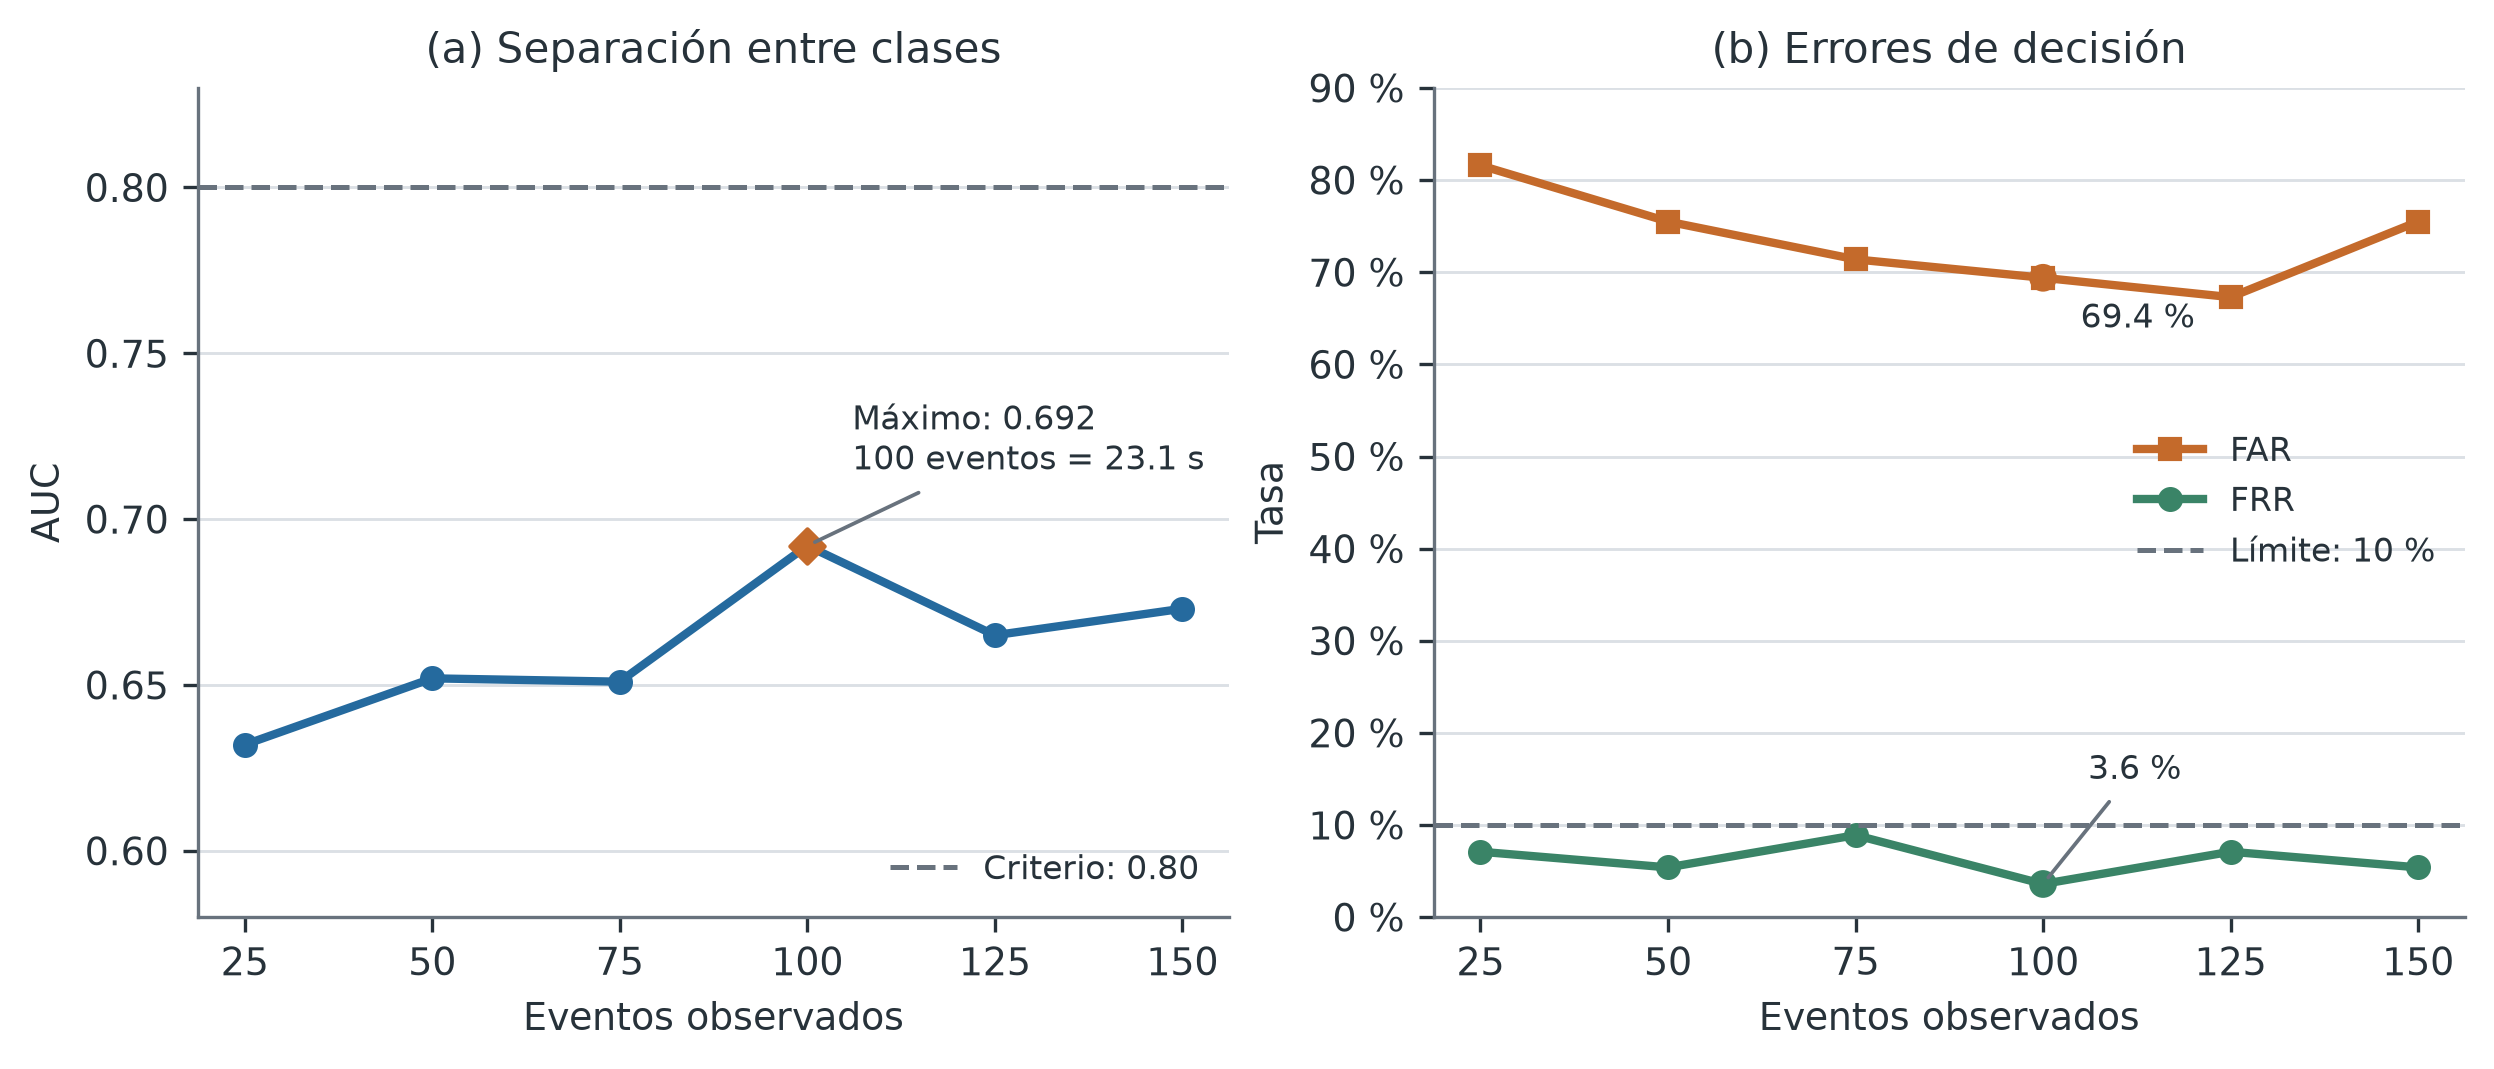
\includegraphics[width=\textwidth]{metricas_por_eventos.png}
  \caption{Evolución del AUC, la FAR y la FRR al aumentar la cantidad de eventos observados. Las líneas discontinuas
  representan los límites establecidos antes de la evaluación.}
  \label{fig:metricas-eventos}
\end{figure}

\subsection{Características con mayor discriminación}

A 100 eventos, las señales individuales más discriminantes fueron la variación de aceleración, la aceleración media
absoluta y la velocidad máxima. En las tres, la mediana fue mayor para las sesiones impostoras. La Tabla
\ref{tab:ranking} presenta las cinco primeras variables.

\begin{table}[htbp]
  \centering
  \caption{Principales características individuales a 100 eventos.}
  \label{tab:ranking}
  \small
  \begin{tabularx}{\textwidth}{Xrrr}
    \toprule
    Característica & AUC orientado & Mediana legítima & Mediana impostora \\
    \midrule
    Variación de aceleración & 0.769 & 4433.022 & 9707.450 \\
    Aceleración media absoluta & 0.743 & 2844.057 & 4809.817 \\
    Velocidad máxima & 0.665 & 3273.308 & 5095.940 \\
    Variación de velocidad & 0.657 & 639.502 & 866.590 \\
    Fracción de movimientos & 0.626 & 0.890 & 0.860 \\
    \bottomrule
  \end{tabularx}
\end{table}

El ranking coincide en dirección general con el antecedente de Antal y Egyed-Zsigmond \cite{antal2019}, que
encontró información relevante en aceleración y \emph{jerk}. No obstante, los valores presentes son diagnósticos
univariados de
un solo usuario y no prueban que esas variables sean universales.

La Figura~\ref{fig:caracteristicas} ordena las cinco variables principales. Las barras comienzan en 0.5, valor que
representa una separación equivalente al azar, para destacar la señal adicional que aporta cada característica.

\begin{figure}[H]
  \centering
  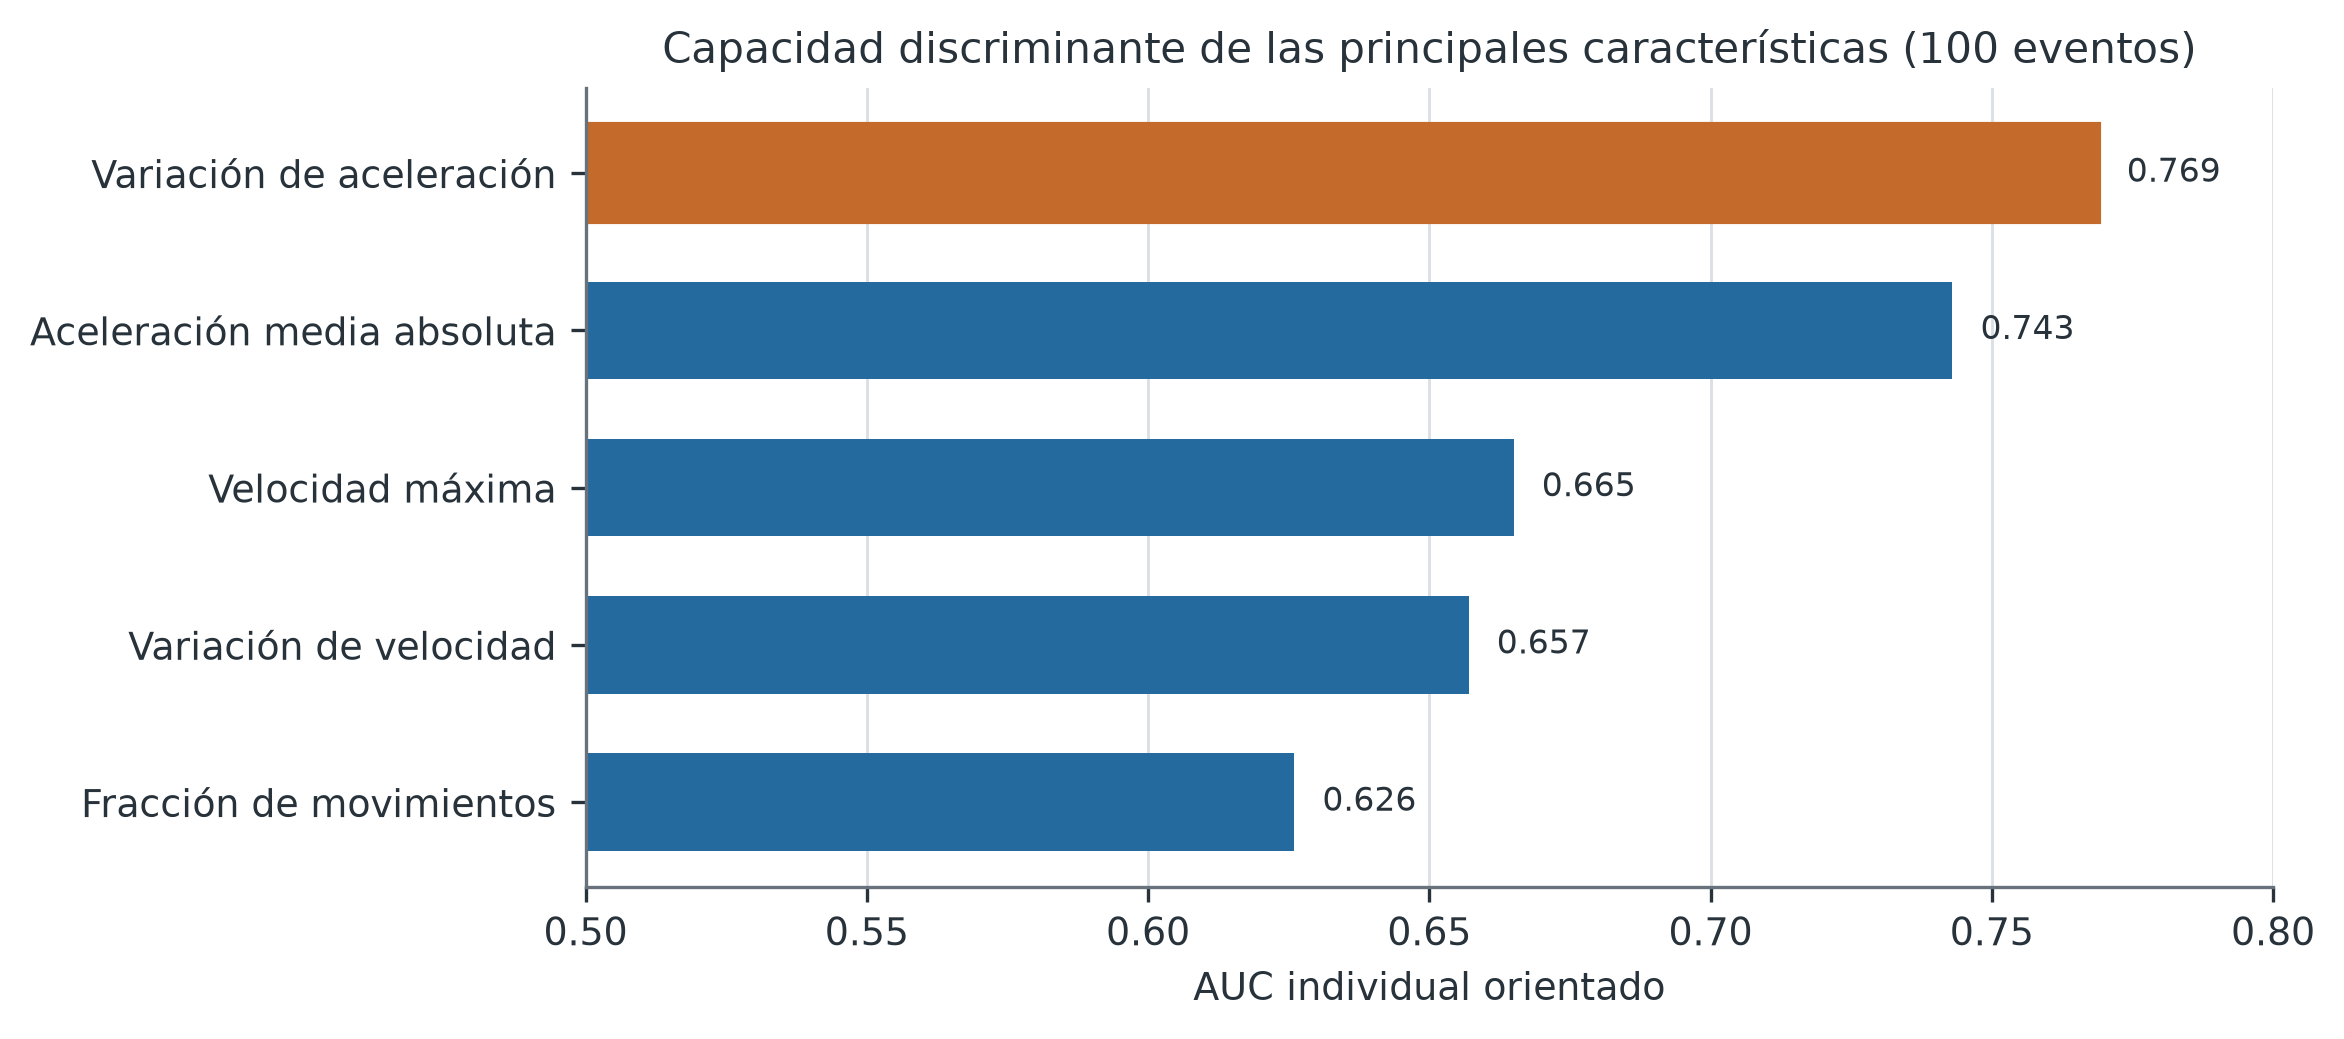
\includegraphics[width=0.94\textwidth]{caracteristicas_discriminantes.png}
  \caption{AUC individual orientado de las características con mayor discriminación a 100 eventos. La variación de
  aceleración produjo la separación individual más alta.}
  \label{fig:caracteristicas}
\end{figure}

\subsection{Estabilidad legítima entre sesiones}

En las siete sesiones legítimas, la tasa de alarma varió entre 6.3\% y 18.0\%. En las dos sesiones reservadas para
validación estuvo entre 7.3\% y 12.5\%. La sesión con mayor tasa pertenecía al propio enrolamiento, lo cual indica
que el
perfil legítimo conserva heterogeneidad aun dentro de los datos disponibles.

\begin{table}[htbp]
  \centering
  \caption{Puntajes legítimos por sesión con ventanas de 100 eventos.}
  \label{tab:estabilidad}
  \small
  \begin{tabular}{llrrr}
    \toprule
    Sesión & Rol & Ventanas & Mediana & Tasa de alarma \\
    \midrule
    2144641057 & Enrolamiento & 300 & 0.397 & 9.0\% \\
    5265929106 & Enrolamiento & 300 & 0.399 & 12.3\% \\
    5815391283 & Enrolamiento & 300 & 0.394 & 6.3\% \\
    7409188284 & Enrolamiento & 300 & 0.429 & 18.0\% \\
    8872593360 & Enrolamiento & 300 & 0.393 & 8.3\% \\
    9031593624 & Validación & 300 & 0.392 & 7.3\% \\
    9838420452 & Validación & 297 & 0.400 & 12.5\% \\
    \bottomrule
  \end{tabular}
\end{table}

La Figura~\ref{fig:estabilidad} muestra que la tasa de alarma cambia incluso entre sesiones legítimas. Una sesión de
enrolamiento llegó al 18.0\%, mientras otras permanecieron por debajo del límite del 10\%.

\begin{figure}[H]
  \centering
  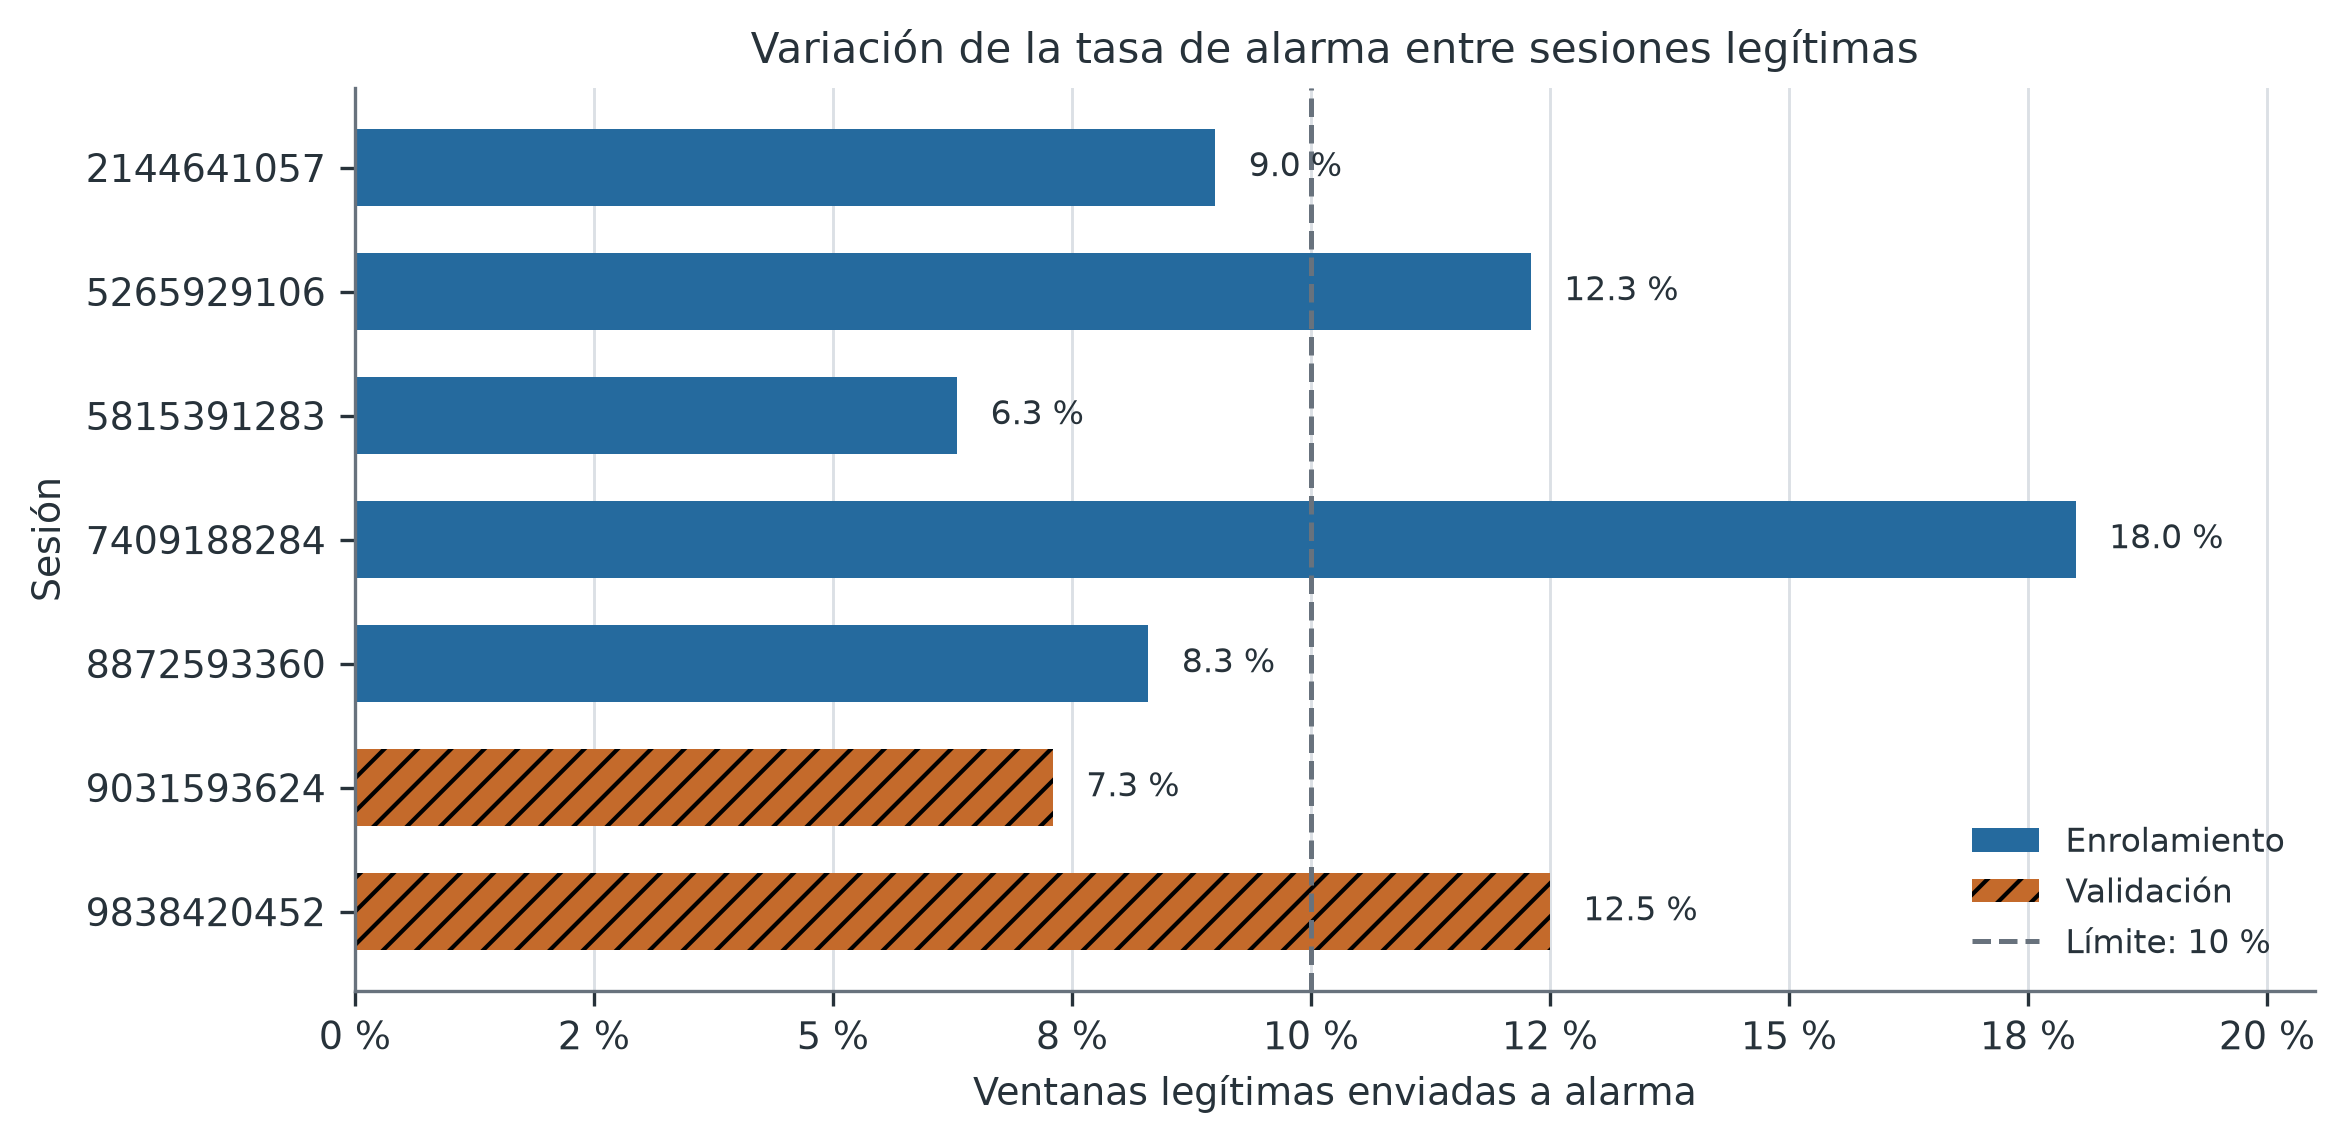
\includegraphics[width=0.94\textwidth]{estabilidad_sesiones.png}
  \caption{Tasa de alarma por sesión legítima con ventanas de 100 eventos. El color y el tramado distinguen las
  sesiones de enrolamiento de las reservadas para validación.}
  \label{fig:estabilidad}
\end{figure}

\section{Discusión}

Los resultados responden las cuatro preguntas de investigación. Primero, las características de aceleración fueron
las
que mejor separaron individualmente las clases a 100 eventos. Segundo, observar más interacciones ayudó hasta cierto
punto, pero el efecto no fue creciente ni suficiente: el mejor AUC apareció en 100 eventos y el menor FAR en 125.
Tercero, no existe un mínimo dentro del rango estudiado porque ninguna configuración satisfizo el criterio declarado.
Cuarto, el comportamiento legítimo no fue completamente estable; la tasa de alarma cambió en 11.7 puntos porcentuales
entre sesiones.

El hallazgo principal no es que 100 eventos sean suficientes, sino que el criterio previo evita presentar como
exitoso un modelo que conserva baja FRR a costa de aceptar a la mayoría de los impostores. El percentil 90 protege
la experiencia del usuario legítimo, pero la superposición entre distribuciones limita la sensibilidad. Bajar el
umbral podría detectar
más impostores, aunque aumentaría las falsas alarmas; subirlo tendría el efecto contrario.

La comparación con CAPTCHA también debe mantenerse dentro del alcance empírico. El conjunto de prueba contiene
suplantaciones simuladas mediante sesiones de otras personas, no agentes de IA ni automatizaciones. Por ello, el
método evalúa continuidad de un patrón personal y podría detectar un agente solo si su interacción resulta
anómala.
Comprobar
esa capacidad exigiría un conjunto específico con distintos agentes, dispositivos, velocidades y estrategias de
imitación.

\subsection{Limitaciones}

\begin{itemize}
  \item El análisis corresponde a una sola cuenta y no estima generalización entre personas.
  \item Las suplantaciones son simuladas; una anomalía no equivale a intención maliciosa.
  \item Solo dos sesiones legítimas fijan el umbral, por lo que la cola de validación puede ser inestable.
  \item Los primeros $N$ eventos producen una decisión temprana única, no vigilancia secuencial en tiempo real.
  \item Cambios de dispositivo, resolución, fatiga, lesión, tarea o contexto pueden alterar el patrón legítimo.
  \item El AUC individual describe asociación y no causalidad ni importancia dentro del modelo multivariado.
\end{itemize}

\subsection{Implicaciones éticas y operativas}

La dinámica de mouse debe tratarse como dato biométrico conductual. Una implementación real requiere
consentimiento, minimización y protección de los registros, límites de retención, auditoría de desempeño y un
mecanismo accesible de
recuperación. La salida apropiada del modelo es una señal de riesgo para autenticación escalonada, no una decisión
irrevocable sobre identidad o culpabilidad.

\section{Conclusiones y trabajo futuro}

La dinámica de mouse ofrece una vía conceptualmente diferente y complementaria a los retos puntuales: permite observar
si la manera de interactuar continúa siendo compatible con el perfil de la persona autenticada. La base científica
explica tanto la estructura de las variables cinemáticas como la necesidad de tolerar variación natural. En el caso
de \texttt{user12}, la aceleración aportó la señal individual más clara y 100 eventos dieron el mejor compromiso
global,
pero la elevada FAR impidió satisfacer el criterio operativo. La conclusión válida es negativa y útil: el prototipo
detecta señal, aunque todavía no ofrece seguridad suficiente para uso autónomo.

El siguiente paso debe ampliar la evaluación a todas las cuentas, estimar incertidumbre mediante remuestreo por
sesión y
calibrar el umbral con validación cruzada entre sesiones legítimas. También conviene comparar ventanas definidas por
tiempo, transformaciones robustas y actualizaciones controladas del perfil. Para estudiar específicamente
suplantación por IA, será necesario recolectar datos de agentes que operen interfaces y evaluar ataques que intenten
imitar al usuario.

\begin{thebibliography}{9}
\raggedright

\bibitem{flash1985}
T. Flash y N. Hogan,
\emph{The coordination of arm movements: An experimentally confirmed mathematical model},
\textit{The Journal of Neuroscience}, vol. 5, núm. 7, pp. 1688--1703, 1985.

\bibitem{dhawale2017}
A. K. Dhawale, M. A. Smith y B. P. Ölveczky,
\emph{The role of variability in motor learning},
\textit{Annual Review of Neuroscience}, vol. 40, pp. 479--498, 2017.
doi: \texttt{10.1146/annurev-neuro-072116-031548}.

\bibitem{antal2019}
M. Antal y E. Egyed-Zsigmond,
\emph{Intrusion detection using mouse dynamics},
\textit{IET Biometrics}, vol. 8, núm. 5, pp. 285--294, 2019.
doi: \texttt{10.1049/iet-bmt.2018.5126}.

\bibitem{liu2008}
F. T. Liu, K. M. Ting y Z.-H. Zhou,
\emph{Isolation Forest},
en \textit{Proceedings of the 8th IEEE International Conference on Data Mining}, pp. 413--422, 2008.

\bibitem{balabit2016}
Balabit,
\emph{Mouse Dynamics Challenge Dataset}, 2016.
Repositorio \texttt{balabit/Mouse-Dynamics-Challenge} en GitHub.

\end{thebibliography}

\end{document}
